\chapter{Miami Wealth, Credibility, and the Arithmetic of Getting to Yes}

This chapter follows a School of Hard Knocks interview, curated by LazyingArt LLC, and treats it as a lecture in commercial reasoning. We begin with yachts, but the first variable the lecture introduces is not capital; it is access. From there the narrative moves through scarcity, sales, sacrifice, survivable risk, value pricing, and finally the slower problem of keeping a real operating company alive. A short early stretch of the transcript is garbled and contributes no stable content, so we follow the usable spine of the lecture and keep the numerical claims explicitly speaker-attributed where the language is approximate.

\section{Wealth Field and the Price of Access}

The lecture opens in spectacle. A stranger is stopped beside a yacht; the host announces a channel with ten million followers; hedge funds, billion-dollar companies, and yacht ownership appear before any theory has been stated. We should not flatten this into mere bravado. The opening teaches a method. In a private field, wealth is not first explained to us; it must be approached, and the approach requires a token of legitimacy.

Miami is then framed as the stage on which this search is being carried out. The lecture presents the city as a dense wealth field, and the numbers are used not as a census table but as the opening coordinates of the search:
\begin{equation}
r_{\mathrm{Miami}} = 6,
\qquad
N_{\mathrm{billionaires}} > 12,
\qquad
F_{\mathrm{host}} = 10\times 10^{6}.
\end{equation}
Here \(r_{\mathrm{Miami}}\) is the host's stated national rank of the city by millionaire count, \(N_{\mathrm{billionaires}}\) is his stated billionaire count, and \(F_{\mathrm{host}}\) is the follower base that functions as an access credential.

The opening cold fragments already hint at the amplitude of the field. One speaker says he has made about \$300 million in a single year; another says his company did about \$8.5 billion last year. The lecture does not yet analyze these claims. It simply places them in front of us so that we feel the size of the terrain before we enter it.

What matters immediately is the doctrine repeated later in the chapter: credibility matters. In this lecture, credibility is not treated as a halo or a virtue word. It is the practical condition under which doors open, suspicion relaxes, and conversation begins.

\section{Lack, Early Labor, and Sales as Empathy}

After the opening spectacle the lecture comes down to ground level. The first substantial entrepreneur says she owns five businesses, that she first became an equity partner at twenty-four, and that she came from nothing: four children, a single mother, food stamps, and a trailer behind her grandparents' house. The lecture now changes register. Wealth is no longer introduced as visible luxury, but as a long response to lack.

The first important transition is from lack to labor. At nine she begins working; by eighteen, while others are only beginning to think about work, she says she has already been at it for a decade. The lecture asks what such an early apprenticeship actually produces, and the answer is not abstract grit alone. It produces usable commercial skill: sales expertise, work ethic, and the habit of moving before one fully knows the map.

\paragraph{Mechanism.}
The lecture gives a compact sales theory. One does not begin with what we want to sell. One begins with what the other person needs solved.

\begin{figure}
\centering
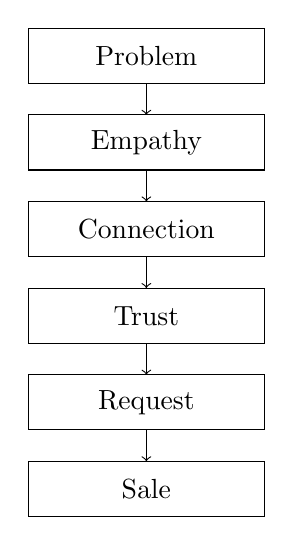
\begin{tikzpicture}[x=1cm,y=1cm]
\draw (0,0) rectangle (3,0.7);
\node at (1.5,0.35) {Problem};
\draw (0,-1.1) rectangle (3,-0.4);
\node at (1.5,-0.75) {Empathy};
\draw (0,-2.2) rectangle (3,-1.5);
\node at (1.5,-1.85) {Connection};
\draw (0,-3.3) rectangle (3,-2.6);
\node at (1.5,-2.95) {Trust};
\draw (0,-4.4) rectangle (3,-3.7);
\node at (1.5,-4.05) {Request};
\draw (0,-5.5) rectangle (3,-4.8);
\node at (1.5,-5.15) {Sale};
\draw[->] (1.5,0) -- (1.5,-0.4);
\draw[->] (1.5,-1.1) -- (1.5,-1.5);
\draw[->] (1.5,-2.2) -- (1.5,-2.6);
\draw[->] (1.5,-3.3) -- (1.5,-3.7);
\draw[->] (1.5,-4.4) -- (1.5,-4.8);
\end{tikzpicture}
\caption{Transcript-derived schematic of the lecture's sales logic.}
\end{figure}

In the lecture's own logic, the sequence is
\begin{equation}
\text{problem} \to \text{empathy} \to \text{connection} \to \text{trust} \to \text{request} \to \text{sale}.
\end{equation}
The crucial step is the middle one. We do not move directly from inventory to sale. We move through the buyer's pain point, and only then does the buyer ask for the solution.

\subsection{Question \& Answer}

Why does empathy sell better than product pushing?

Because the lecture does not treat a sale as the triumph of pressure. It treats a sale as the moment when the other person recognizes that we understand the problem from the inside. If we begin with ``Here is what I want you to have,'' we remain trapped on our side of the table. If we begin by locating the other person's difficulty, naming it, and speaking to it in their language, then trust is created before persuasion is attempted. In the lecture's vocabulary, that is how the ask becomes natural rather than forced.

\section{Sacrifice, Mobility, and Fearful Resistance}

The lecture does not allow this sales module to float free of cost. Immediately after the masterclass comes the bill. We are told of four years without a single day off, no vacations, friends marrying and having children, and a move from Boston to Saginaw, Michigan, a place presented not as glamorous opportunity but as commercial obscurity. The point is sharp: credibility is not only granted from above; it is also built from below by choosing difficult ground and staying on it.

This matters because the lecture does not romanticize the climb as a cleanly heroic story. It introduces a second obstacle. The people who slow us down need not be declared enemies. They may love us. They may simply be afraid.

\subsection{Question \& Answer}

Are the people holding us back always enemies?

The lecture answers no. Sometimes the friction comes from hatred, but sometimes it comes from care distorted by fear. Loved ones may try to pull us back not because they want our failure, but because they cannot imagine our path without danger. That is why the lecture insists on a more difficult move than denunciation. We acknowledge the fear, thank the person, and move anyway. In this part of the chapter the real asymmetry is between borrowed fear and private judgment. No one else, the speaker says, can know what is best for us in the way we ourselves must know it.

This is an important narrative beat. Wealth is no longer opposed only by market difficulty. It is opposed by social gravity. The lecture keeps that gravity human, and therefore harder to dismiss.

\section{Risk, Drawdown, Networking, and Speed}

The setting now changes. We are taken to the Miami Beach Yacht Harbor, and the lecture again makes us feel the gate: private docks, private offices, refusal at the entrance, and then eventual access. Once inside, the scale of the story changes from bootstrap labor to institutional finance. A hedge-fund operator describes nearly three decades in the business, thousands of traders, hundreds of employees, and a measurable fraction of market volume:
\begin{equation}
T_{\mathrm{fund}} \approx 28\,\mathrm{yr},
\qquad
N_{\mathrm{traders}} \approx 4000,
\qquad
N_{\mathrm{emp}} \approx 600,
\qquad
s_{\mathrm{mkt}} \approx 0.03\text{--}0.04.
\end{equation}
These numbers are speaker-attributed and approximate, but their purpose is plain. The lecture is no longer speaking about an ambitious individual learning to sell; it is speaking about a machine.

Then comes the cleanest loss event in the lecture: a little over \$8 million lost in a single day.
\begin{equation}
L_{\mathrm{day}} \gtrsim \$8\times 10^{6}.
\end{equation}
The important thing is not the drama of the number itself. The important thing is the rule extracted from it. The speaker says that after such a day he learned to know his risk and to choose only the amount he could afford to see go to zero.

\begin{definition}
A risk choice is \emph{survivable} if a total loss of the position still leaves the investor or operator able to continue.
\end{definition}

If \(I\) is the capital committed to a position, then the lecture's rule can be written in minimal form as
\begin{equation}
W_{\mathrm{after}} = W_{\mathrm{before}} - I,
\end{equation}
with \(I\) chosen so that \(W_{\mathrm{after}}\) remains a balance sheet we can live with even in the failure state.

\subsection{Question \& Answer}

How much risk can we actually afford to take?

Not the amount that flatters the ego, and not the amount suggested by momentary confidence. The lecture's answer is more austere. We can take only the amount whose complete destruction does not destroy us. This is not timidity. It is continuity. The point is not to avoid exposure altogether, but to keep failure from becoming terminal.

The lecture then turns from risk to relationships. The host asks whether the richest people on Wall Street always make money by placing trades. The answer opens a second mechanism: networking. A contact made at a golf tournament is followed up immediately, the man is brought in to see the company, he becomes chairman, and the company pivots upward. The sequence is worth writing as a process:
\begin{equation}
\text{contact} \to \text{immediate call} \to \text{meeting} \to \text{chairmanship} \to \text{pivot}.
\end{equation}
What matters here is the fusion of two claims. Speed matters, but speed by itself is empty. The call must be immediate, and there must also be something real to show when the door opens. The lecture is careful on this point. Access without substance is noise; substance without timely motion remains unseen.

The same speaker then shifts into the language of mindset and manifesting. We should not inflate that language into a theorem it is not trying to be. In the lecture it means something concrete: imagine the objective, enumerate the steps, and move without delay. The mystical vocabulary is present, but the operative content is disciplined action.

\section{Credibility, Systems, and the Dollar Value of Time}

Before the next interview, the lecture inserts a short operating maxim. Companies, we are told, die from indigestion and starvation. The line is memorable because it puts two kinds of failure on the same page. A firm can die because it never secures enough business, but it can also die because growth outruns systems, inventory, accounting, and control. This aside does not dominate the chapter, but it belongs here because it prepares us to read the next interview as an argument not only about selling, but about the commercial value of speed inside a real operating system.

The next speaker is introduced through the line ``credibility matters.'' Again the host uses his own audience size to gain a minute of attention. That minute yields one of the lecture's sharpest business fragments: a founder who helps companies navigate regulatory and clinical pathways, whose company he says did roughly \$8.5 billion last year,
\begin{equation}
R_{\mathrm{company}} \approx \$8.5\times 10^{9},
\end{equation}
and who condenses selling into a sentence of striking economy: he does not sell; he finds out what the client needs and hits the client's goal.

This is the chapter's clearest moment of value arithmetic. The interview moves from ego to sales and then from sales to pricing. The speaker asks: if I can get your product to market faster than you can, what is that worth to you? A specific example follows. Suppose the product would do \$12 million in a year, and suppose the launch can be accelerated by three months.

\begin{proposition}
Under the lecture's linear-accrual heuristic, if a product would produce \(R_{\mathrm{year}} = \$12\,\mathrm{M}\) in a year and the launch is accelerated by \(\Delta t = 3\) months, then the gross incremental value created for the buyer is \(\Delta V = \$3\,\mathrm{M}\).
\end{proposition}

\begin{proof}
We first convert annual revenue to monthly revenue:
\begin{align}
R_{\mathrm{month}}
&= \frac{R_{\mathrm{year}}}{12}
= \frac{\$12\,\mathrm{M}}{12}
= \$1\,\mathrm{M/month}.
\end{align}
Now multiply by the time saved:
\begin{align}
\Delta V
&= R_{\mathrm{month}} \Delta t
= (\$1\,\mathrm{M/month})(3\,\mathrm{months})
= \$3\,\mathrm{M}.
\end{align}
\end{proof}

If the fee is \$300{,}000, the lecture then invites the simplest comparison:
\begin{align}
F &= \$300{,}000,\\
S_{\mathrm{buyer}} &= \Delta V - F = \$3{,}000{,}000 - \$300{,}000 = \$2{,}700{,}000,\\
\frac{\Delta V}{F} &= 10.
\end{align}
So the fee is one tenth of the gross buyer-side value created by the acceleration, and the buyer's gross surplus is \$2.7 million.

\subsection{Question \& Answer}

Why is a \$300{,}000 fee cheap if it creates \$3 million in value?

Because in the lecture's logic, price must be judged against buyer-side gain, not against the seller's labor time alone. The service is cheap if it moves the buyer across a large value gap. The point is not that every consulting fee may be justified by bold arithmetic. The point is that negotiation becomes intelligible only when we ask what outcome is being purchased. In this chapter, faster market entry is not a vague promise; it is monetized time.

A caution belongs here. This is gross-value arithmetic, not a complete profit-and-loss model. The lecture does not pause to account for margins, adoption lag, or regulatory contingencies. Still, its commercial insight is clear. Time can be priced when time moves revenue.

The same interview closes with another strong claim: the speaker says he has lost everything and rebuilt four times. When pressed for the secret, he does not offer a new widget each time. He says the policies and procedures are the same: treat people right, do what they are looking for, and outwork everybody else. That is the lecture's version of invariance. The objects change; the method does not.

\section{Keeping the Machine Alive}

The final interview narrows the scale. We leave billion-dollar revenue and return to a field-service business run by a mechanical engineer. He says the company has been operating for twenty-two years, that it did about \$30 million in sales last year, and that profit was about \$2 million to \$3 million. At once the lecture shifts from wealth as spectacle to wealth as retained strain. Money is coming through the system, but much of it is going back into the business.

If we write the speaker's numbers in the simplest operating form,
\[
R_{\mathrm{field}} \approx \$30\,\mathrm{M},
\qquad
\Pi_{\mathrm{field}} \approx \$2\text{--}3\,\mathrm{M},
\]
then the implied margin band is
\begin{equation}
m = \frac{\Pi_{\mathrm{field}}}{R_{\mathrm{field}}}
\approx \frac{2}{30}\text{--}\frac{3}{30}
\approx 0.067\text{--}0.10.
\end{equation}
So the lecture closes not with an easy story of cash extraction, but with a thinner operating spread and a reinvestment burden.

The bottleneck, we are told, is labor. The firm cannot scale without good employees, and good employees are difficult to find. That claim is then embedded in a larger picture. The most important hire so far is a twin brother. The father trained them into the business. Physical discipline matters; gym routine is presented as a cousin of work routine. Down cycles happen. It is easy to buy the visible pleasures of a good year; it is harder to step downward when the cycle turns against us.

\subsection{Question \& Answer}

Why is keeping a company harder than starting one?

Because starting is an event, while keeping is a repeated negotiation with labor, cost, family, and appetite. The lecture's final owner describes exactly this burden. We must keep employees, keep standards, keep reinvestment going, keep our household aligned with the business cycle, and keep ourselves from building a lifestyle that cannot survive a bad year. What is difficult is not merely ignition. It is sustained combustion.

This is also where the lecture places a final distinction between entrepreneurship and employment. Not everyone, the speaker says, is built for entrepreneurship. Some people are great employees. The point is not to rank these lives morally. It is to note the structure of sacrifice. Entrepreneurship demands irregular pressure not only from the owner but from spouse, children, travel schedule, and tolerance for uncertainty.

\section{Summary}

We can now see the chapter's progression clearly. It begins with access, because without access the rest of the lecture cannot even occur. It then moves to a bootstrap account of labor and sales, where we are taught that selling is diagnosis plus trust rather than pressure. From there it prices the climb in terms of sacrifice and social resistance. Only after that moral and practical groundwork has been laid does the lecture turn to institutional scale, one-day losses, survivable risk, networking, and the necessity of speed.

The later sections sharpen these themes into commercial arithmetic. Credibility opens the conversation. Ego can ruin a firm. Time-to-market has a dollar value. A fee becomes intelligible when we compare it with the value gap it closes. Finally, the lecture descends again from the height of billion-dollar claims to the slower mathematics of operating margin, hiring friction, reinvestment, and cyclic durability. The result is not a theory of wealth in the abstract. It is a sequence of local rules: get in the room, understand the other person's need, risk only what can die without killing you, move while the opportunity is warm, and build a machine that can survive its own growth.